\chapter{Templates}\label{chap:format}

\section{Introduction}
The format is adapted from the Format for the Preparation of Scientific and Technical Reports, Dissertations and Academic Theses of the People's Republic of China and the Dissertation Format of Northeastern University, and is designed for use by applicants for master's and doctoral degrees in writing printed dissertations. This format has been implemented since its release.
\section{Main Body of the Thesis}
The main part of the dissertation consists of a front part, a main body, and an ending.
\subsection{Front part}
\begin{itemize}
    \item Cover
    \item Title page - Title page (both Chinese and English)
    \item Declaration (Statement of Originality)
    \item Abstract (both Chinese and English)
    \item Comments
    \item List of illustrations and schedules (only if necessary)
    \item List of abbreviations, acronyms, symbols, units (only if necessary)
    \item Glossary of terms (only if necessary)
\end{itemize}

\subsection{Main body}
\begin{itemize}
    \item Introduction or preface
    \item Main body
    \item Discussion, conclusions, and recommendations
\end{itemize}
\subsection{Ending (only if necessary)}
\begin{itemize}
    \item References
    \item Acknowledgment
    \item Academic achievements during doctoral studies
    \item The author's resume of scientific research and study experience
    \item Available Bibliographic Titles (only if necessary)
    \item Index (only if necessary)
\end{itemize}

\section{Format}
Paper size: The paper size is standard A4 copy paper (210mm x 297mm).

Edition core (print size): 160mm × 247mm (excluding the header line, page number line).

The font size of the text: small 4 Song, English Times New Roman, uniform throughout the text.

30 to 35 lines per page, 35 to 38 words per line.

Binding: double-sided printing, binding along the long side.

Page numbering: Page numbering in Arabic numerals, the same font size as the text, centered at the bottom of the page, with a dot or a horizontal line on both sides of the number, such as -3- or -3-.

Header: From the abstract page, add a header, which can be single or double line (second line, Wenwu line), with the header description in italics No. 5, "Master's and doctoral dissertation of Northeastern University" at the left end and "Chapter number and title" at the right end.

Cover: The standard cover (double A4) of the dissertation of graduate students (doctoral or master's degree) of Northeastern University.

\section{Style}

\subsection{Title}

The body of the thesis is graded according to chapters, articles, paragraphs and items, and the Arabic numbers of chapters, articles, paragraphs and items at different levels are separated by a dot "." (half-cornered solid lower dot), and no dot after the final number. Layout format see Table 4.1.

This hierarchical numbering method only to the fourth level. Further subdivision can be used (1), (2) ......; (a), (b) ......, etc.

\begin{table}[htpb]
    \begin{center}
        \bicaption{标题排版格式}{Typesetting format of the heading}
        \begin{tabular}{|l | l | l | l |}
            \hline
            Title       & Font   & Format        & Example           \\
            \hline
            Level 1 (chapter) & 2 bold & centered, occupying 3 lines & Chapter 1 XXX \\
            \hline
            Level 2 (article) & 3 bold & centered, 2 lines & 1.1 XXXXXX \\
            \hline
            Level 3 (paragraph) & 4 bold & left, 2 lines & 1.1.1 XXXXXX \\
            \hline
            Level 4 (item) & small four-point bold & left, 1 line & 1.1.1.1 XXXXXX  \\
            \hline
        \end{tabular}
    \end{center}
\end{table}

The abstract, table of contents, references, acknowledgements, academic achievements during the doctoral studies, and biography are laid out as first-level headings.

\subsection{Main body}
Chinese character font size: body font small 4 Song.

Foreign language, digital font size and peer Chinese font size of the same, font with WORD system Time New Roman body or similar fonts.

\subsubsection{Figure}
Illustrations include diagrams, schematics, construction diagrams, curves, block diagrams, flowcharts, layout diagrams, maps, photographs, plates, etc. Illustrations indicate items such as diagram number, diagram title, and legend. Figure number code with the chapter number. For example, "Figure 2.1" means the first figure in Chapter 2. Figure number and the text of the figure title placed between a word space, placed directly below the figure, the figure title with 5 words, font available in Song, shall be unified throughout the text. The text size of the symbols in the figure is not larger than the font size of the figure title.

The insertion of pictures in the paper is usually divided into a single figure and multiple figures, which are described below:

Single image insertion: Suppose the insertion name is \verb|tc_q_criteria|(the suffix can be .jpg, .png, .pdf, the same below) of the image, the effect as shown in the figure:
\ref{fig:tc_q_criteria}。
\begin{figure}[!htbp]
    \centering
    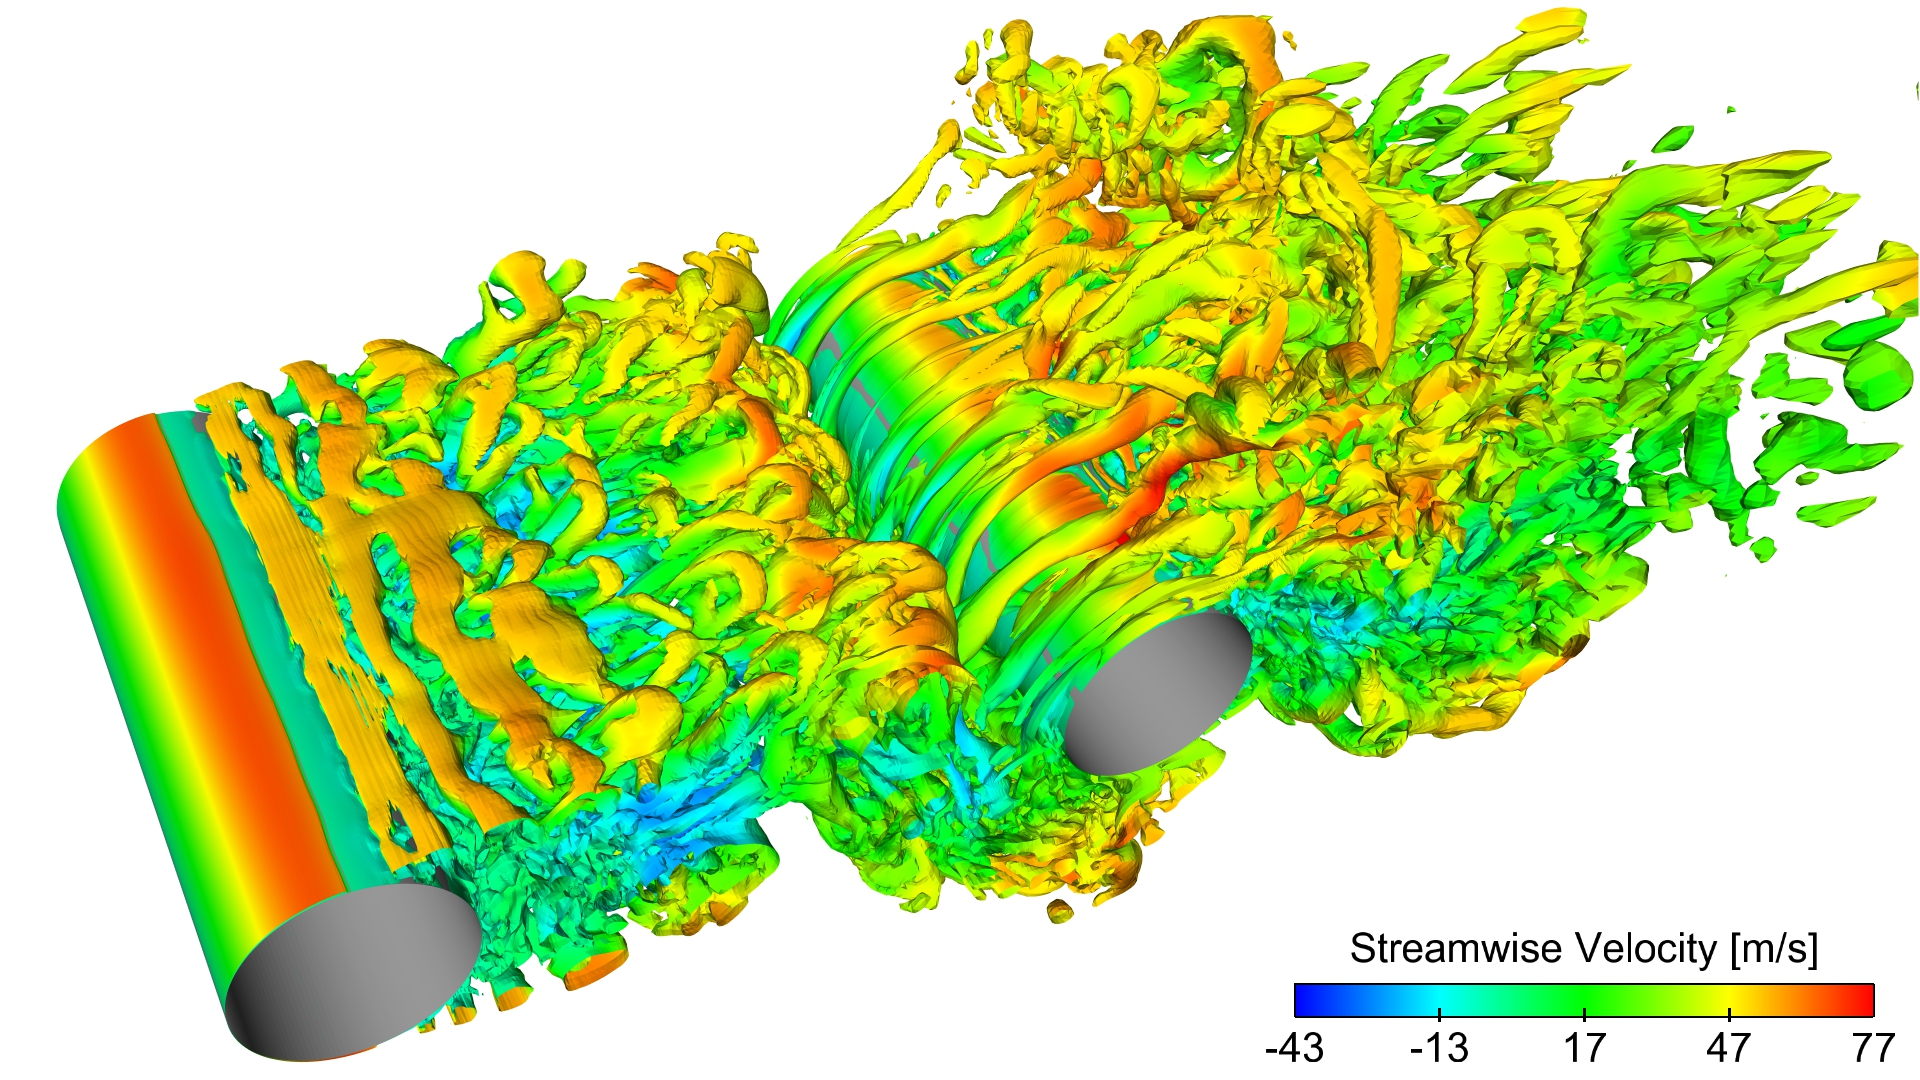
\includegraphics[width=0.40\textwidth]{tc_q_criteria}
    \bicaption{Q判据等值面图,同时测试一下一个很长的标题,比如这真的是一个很长很长很长很长很长很长很长很长的标题。}{Isocontour of Q criteria, at the same time, this is to test a long title, for instance, this is a really very long very long very long very long very long title.}
    \label{fig:tc_q_criteria}
\end{figure}

If the blank area of the illustration is too large,such as \verb|shock_cyn|, will automatically crop to \ref{fig:shock_cyn}.
\begin{figure}[!htbp]
    \centering
    %trim option's parameter order: left bottom right top
    % 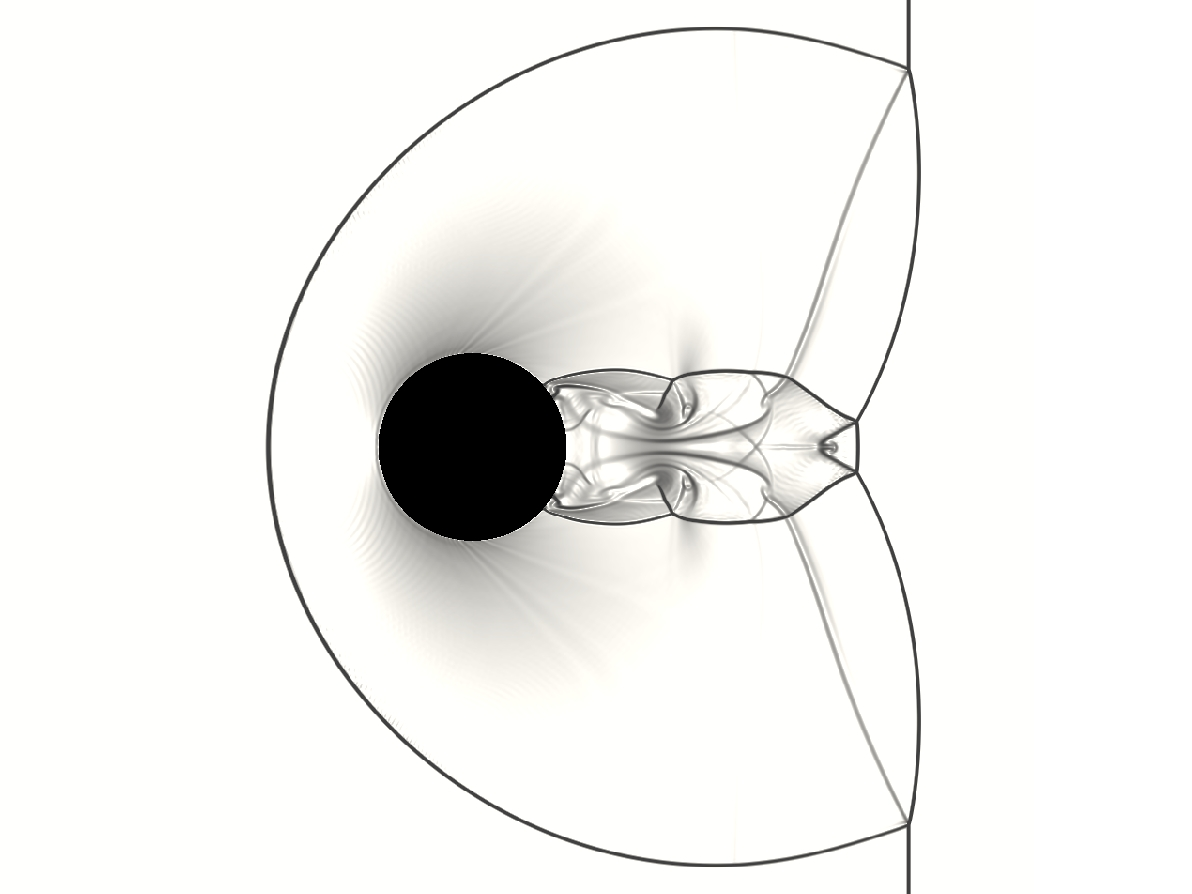
\includegraphics[trim = 30mm 0mm 30mm 0mm, clip, width=0.40\textwidth]{shock_cyn}
    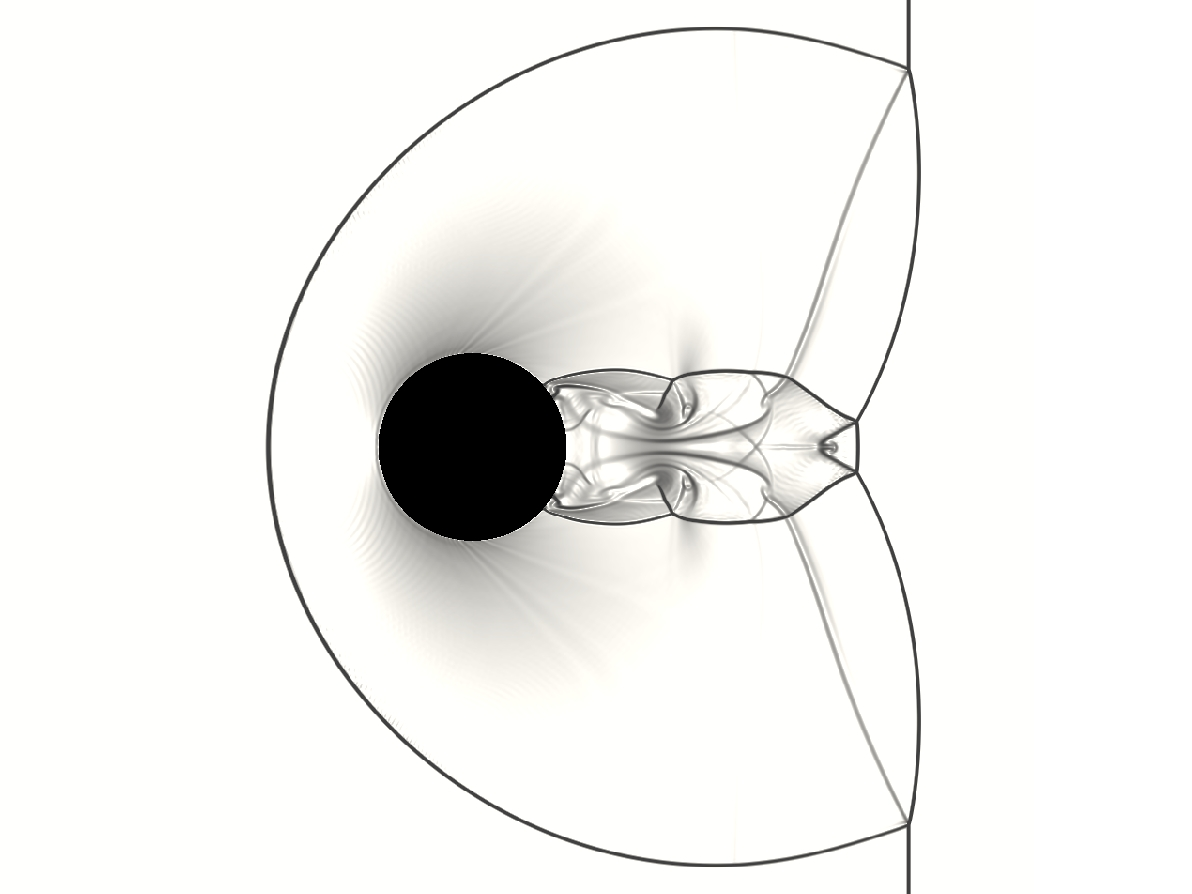
\includegraphics[width=0.40\textwidth]{shock_cyn}
    \bicaption{激波圆柱作用。}{Shock-cylinder interaction.}
    \label{fig:shock_cyn}
\end{figure}

The insertion of multiple figures as Figure \ref{fig:oaspl}, multiple figures should not be given text sub-titles in the sub-figures, as long as the serial number is given, and the main title is cited in the description.
\begin{figure}[!htbp]
    \centering
    \begin{subfigure}[b]{0.35\textwidth}
      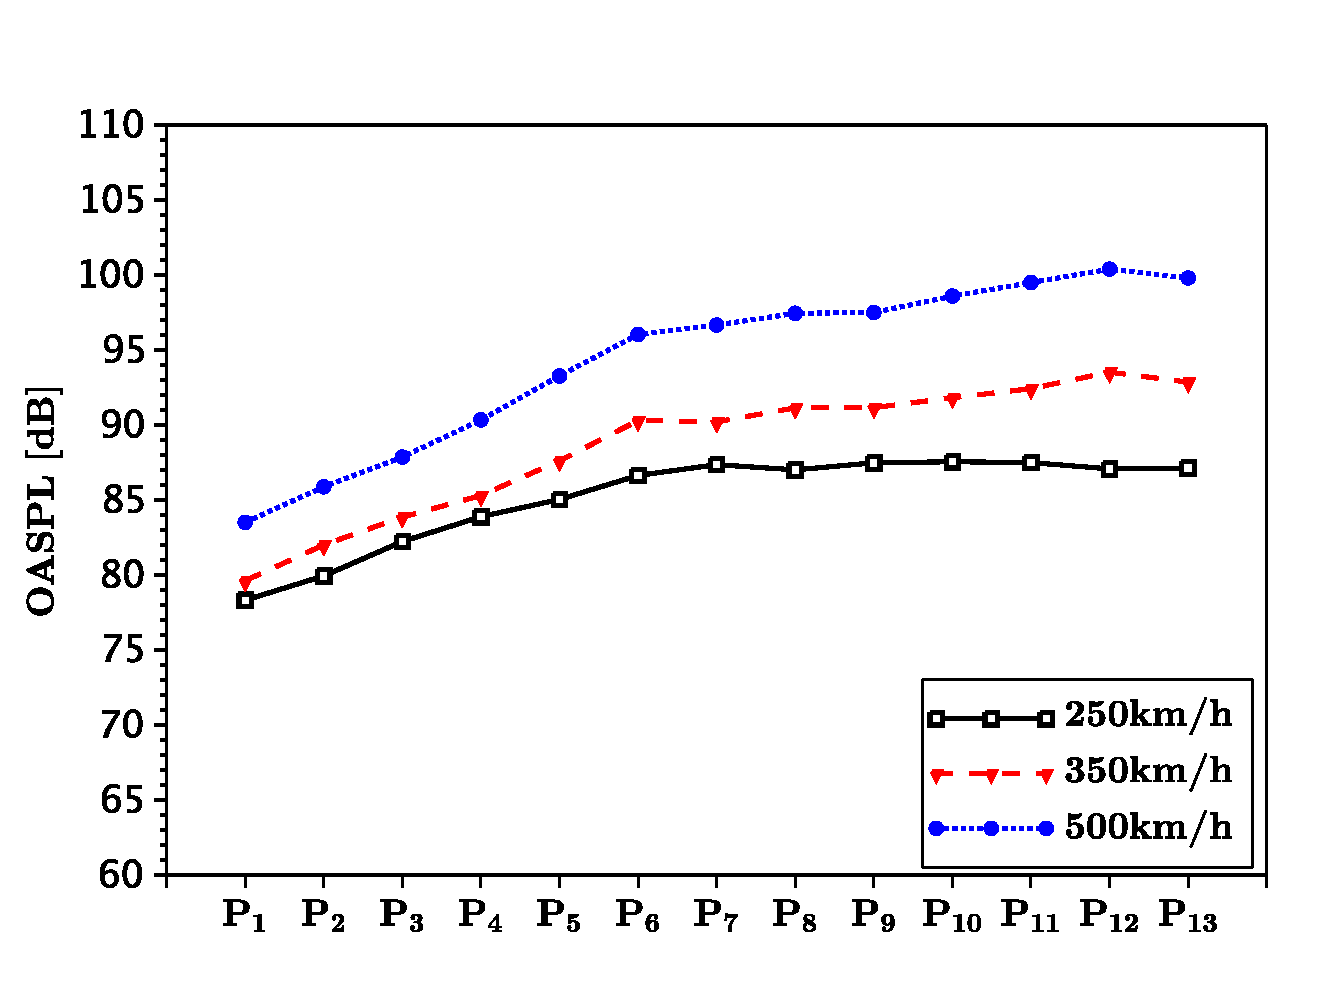
\includegraphics[width=\textwidth]{oaspl_a}
      \caption{}
      \label{fig:oaspl_a}
    \end{subfigure}%
    ~%add desired spacing
    \begin{subfigure}[b]{0.35\textwidth}
      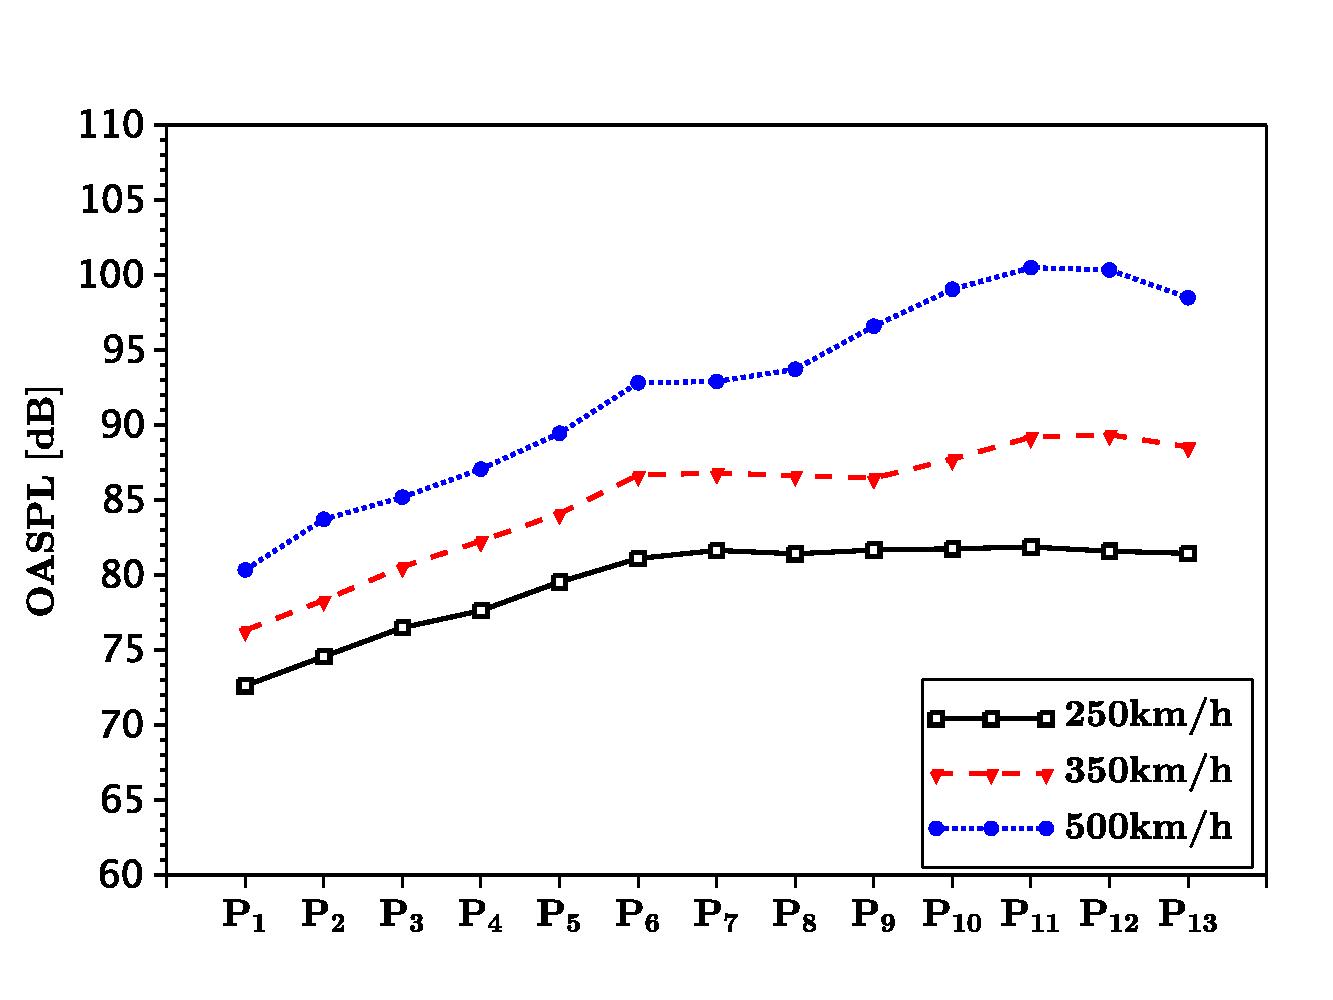
\includegraphics[width=\textwidth]{oaspl_b}
      \caption{}
      \label{fig:oaspl_b}
    \end{subfigure}
    \begin{subfigure}[b]{0.35\textwidth}
      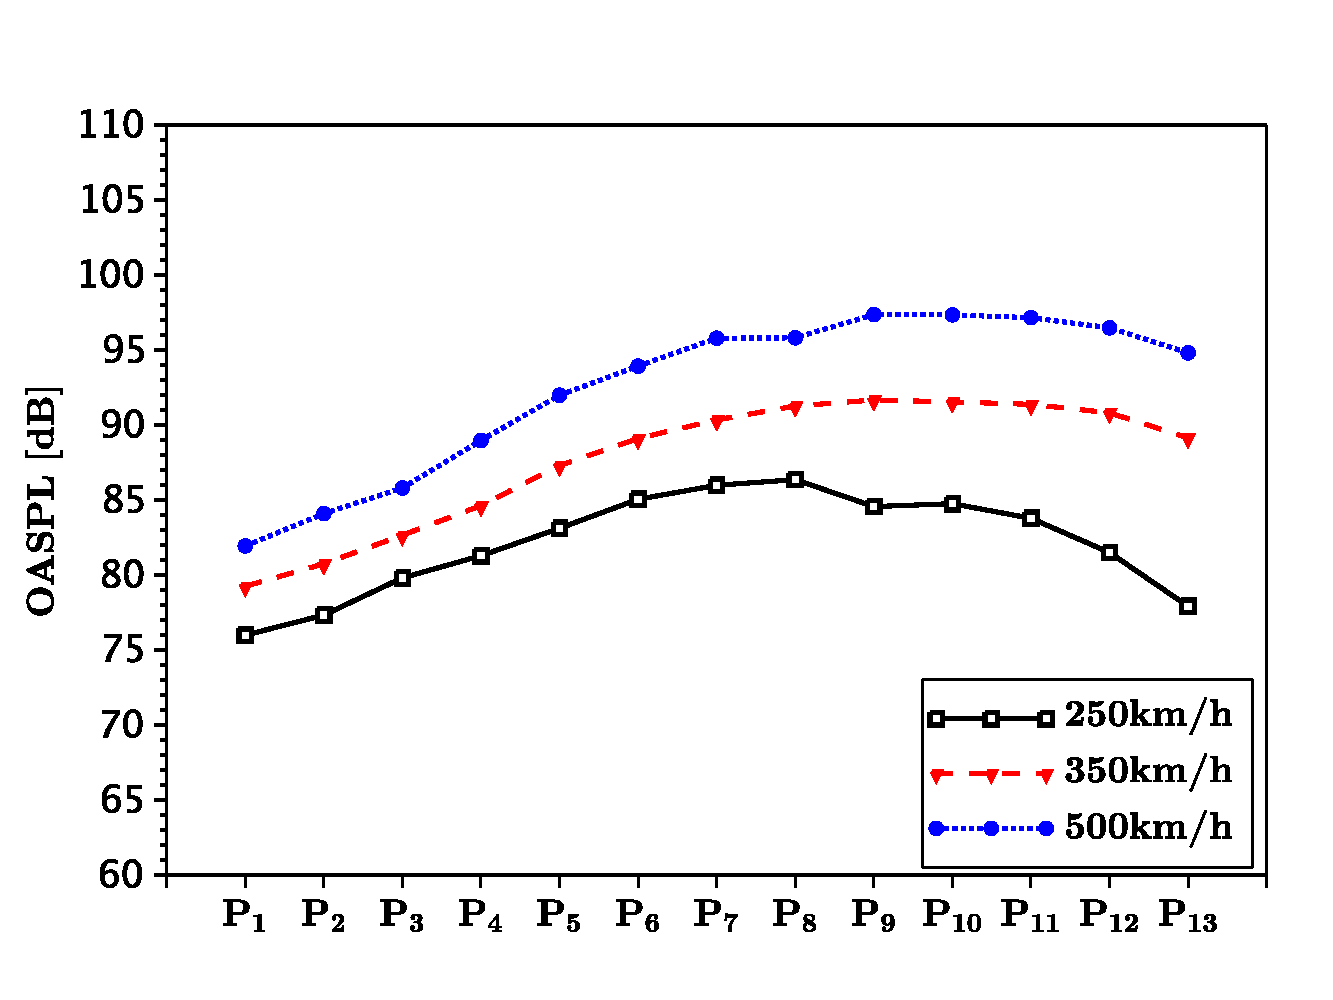
\includegraphics[width=\textwidth]{oaspl_c}
      \caption{}
      \label{fig:oaspl_c}
    \end{subfigure}%
    ~%add desired spacing
    \begin{subfigure}[b]{0.35\textwidth}
      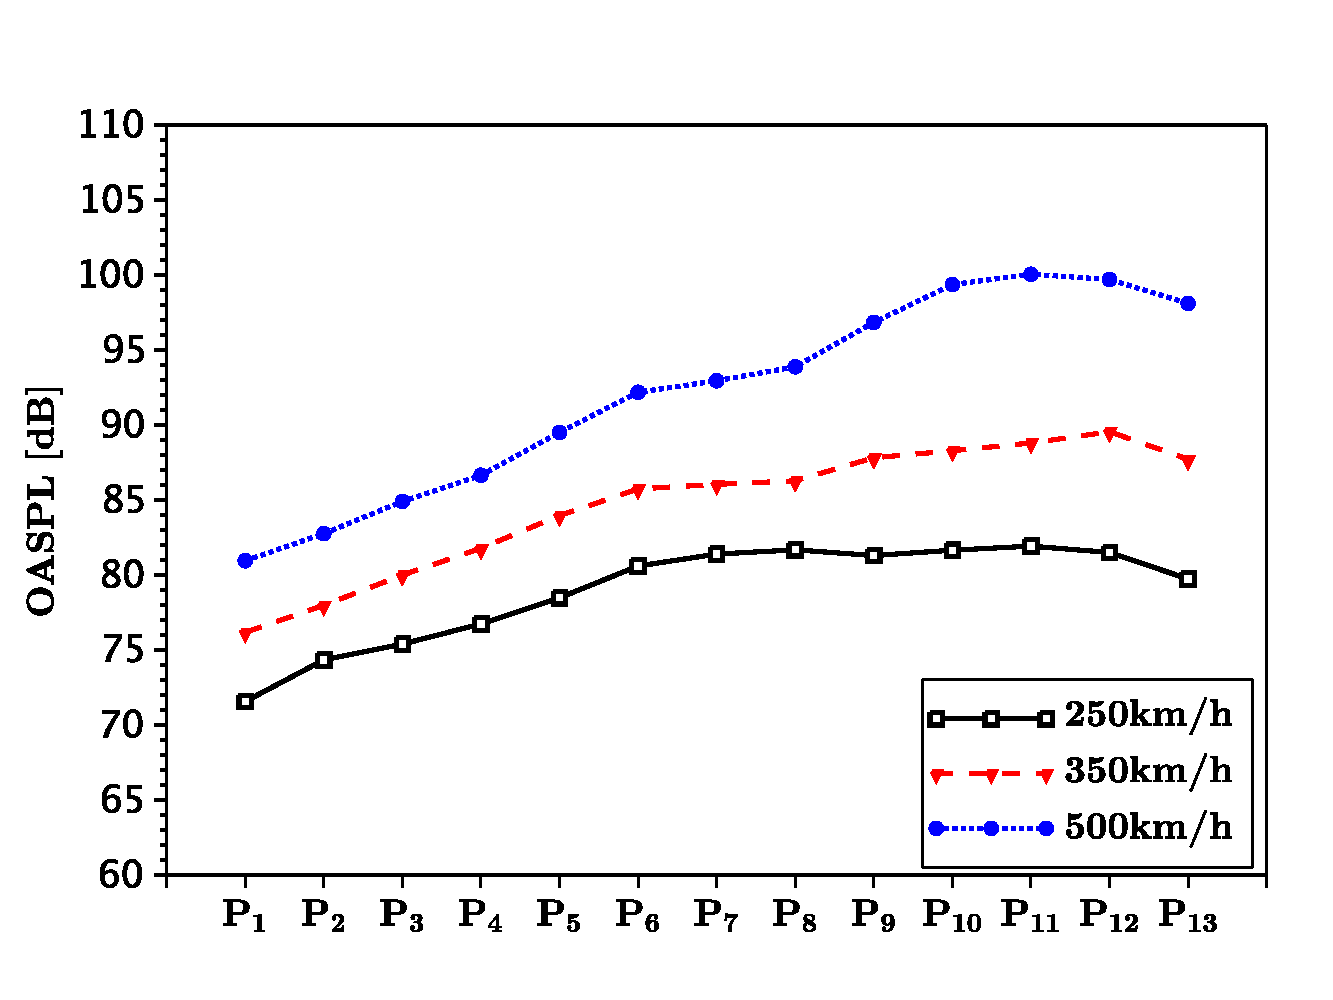
\includegraphics[width=\textwidth]{oaspl_d}
      \caption{}
      \label{fig:oaspl_d}
    \end{subfigure}
    \bicaption{总声压级。(a) 这是子图说明信息,(b) 这是子图说明信息,(c) 这是子图说明信息,(d) 这是子图说明信息。}{OASPL.(a) This is the explanation of subfig, (b) This is the explanation of subfig, (c) This is the explanation of subfig, (d) This is the explanation of subfig.}
    \label{fig:oaspl}
\end{figure}

\subsubsection{Table}
The general format of the table is that the data are arranged vertically in order, and the content and items are read horizontally from left to right in a through layout. Table number is also coded with chapter number, e.g., Table 2.1 is the first table in Chapter 2. Table should have a table title, and table number between the empty 1 to 2 words, placed at the top of the table centered, with 5 Song font, shall be unified throughout the text. Table content and items in the font size is not larger than the font size of the figure title.

Please see table ~\ref{tab:sample}. For more examples of table making, please see  \href{https://en.wikibooks.org/wiki/LaTeX/Tables}{WiKibook Tables}。
\begin{table}[!htbp]
    \bicaption{这是一个样表。}{This is a sample table.}
    \centering
    \footnotesize% fontsize
    \setlength{\tabcolsep}{4pt}% column separation
    \renewcommand{\arraystretch}{1.2}%row space 
    \begin{tabular}{lcccccccc}
        \hline
        Row number & \multicolumn{8}{c}{This is a multicolumn} \\
        %\cline{2-9}% partial hline from column i to column j
        \hline
        Row 1 & $1$ & $2$ & $4$ & $5$ & $6$ & $7$ & $8$\\
        Row 2 & $1$ & $2$ & $4$ & $5$ & $6$ & $7$ & $8$\\
        Row 3 & $1$ & $2$ & $4$ & $5$ & $6$ & $7$ & $8$\\
        Row 4 & $1$ & $2$ & $4$ & $5$ & $6$ & $7$ & $8$\\
        \hline
    \end{tabular}
    \label{tab:sample}
\end{table}


\subsubsection{Equation}
Formulas include mathematical, physical and chemical formulas. Formulas, equations or equations cited in the text can be numbered by chapter number with Arabic numerals (formula number), such as: formula (2.1) that the first chapter 2, formula is generally a single line centered layout and the context is separated, formula number and formula peer right layout.

For example, Navier-Stokes equation: 

\begin{equation} \label{eq:ns}
    \begin{cases}
        \frac{\partial \rho}{\partial t} + \nabla\cdot(\rho\Vec{V}) = 0 \ \mathrm{times\ font\ test}\\
        \frac{\partial (\rho\Vec{V})}{\partial t} + \nabla\cdot(\rho\Vec{V}\Vec{V}) = \nabla\cdot\Tensor{\sigma} \ \text{times font test}\\
        \frac{\partial (\rho E)}{\partial t} + \nabla\cdot(\rho E\Vec{V}) = \nabla\cdot(k\nabla T) + \nabla\cdot(\Tensor{\sigma}\cdot\Vec{V})
    \end{cases}
\end{equation}
\begin{equation}
    \frac{\partial }{\partial t}\int\limits_{\Omega} u \, \mathrm{d}\Omega + \int\limits_{S} \unitVector{n}\cdot(u\Vec{V}) \, \mathrm{d}S = \dot{\phi}
\end{equation}

For common commands for mathematical formulas, see \href{https://en.wikibooks.org/wiki/LaTeX/Mathematics}{WiKibook Mathematics}。artracom.sty encapsulates some common data types such as vector matrices. The advantage of this is that if you need to modify the display form of a vector one day, you only need to modify the vector definition in artracom.sty separately to achieve the full document modification.

\subsubsection{Algorithm}

Please see \ref{alg:euclid}, for more detail, please see \href{https://ctan.org/pkg/algorithmicx?lang=en}{algorithmicx}。

\begin{algorithm}[!htbp]
    \small
    \caption{Euclid's algorithm}\label{alg:euclid}
    \begin{algorithmic}[1]
        \Procedure{Euclid}{$a,b$}\Comment{The g.c.d. of a and b}
        \State $r\gets a\bmod b$
        \While{$r\not=0$}\Comment{We have the answer if r is 0}
        \State $a\gets b$
        \State $b\gets r$
        \State $r\gets a\bmod b$
        \EndWhile\label{euclidendwhile}
        \State \textbf{return} $b$\Comment{The gcd is b}
        \EndProcedure
    \end{algorithmic}
\end{algorithm}

\subsection{Appendix}
The figures, tables, formulas, references, etc. in the appendix are numbered separately from the text, and are also numbered with Arabic numerals, but crowned with the appendix serial number before the digital. For example: Figure A.1, equation (B.3), etc.
\subsection{Unit of measurement}
The dissertation will always adopt the "Legal Units of Measurement of the People's Republic of China" issued by the State Council on February 27, 1984, and follow the "Methods of Using Legal Units of Measurement of the People's Republic of China". The various quantities, units and symbols used for naming in the dissertation must follow the provisions of national standards GB3100-82, GB3101-82, GB3102/1-13-82, etc.

The way of writing unit names and symbols can adopt international common symbols or use Chinese names, but adopt one uniformly and do not mix them.

\subsection{References}

The reference citation process is introduced with an example, assuming the need to cite the document named "Document Preparation System", and the steps are as follows:

1) Use Google Scholar to search for Document Preparation System, click Cite under the target entry, expand it and select Import into BibTeX to open the BibTeX index information of this article, and copy and add them to the ref.bib file (this file is located in the Biblio folder).

2) The first line of the index \verb|@article{lamport1986document,| in \verb|lamport1986document| that is, the label of this document (\textbf{Chinese document must also use the English label}, generally follow: surname pinyin + year + the format of the first word of the title pinyin), want to index this document in the paper, there are two types of indexing:

Text type: \verb|\citet{lamport1986document}|. As shown here \citet{lamport1986document}. 

Bracket type: \verb|\citep{lamport1986document}|. as shown here \citep{lamport1986document}.

\textbf{multi-document index separated by English commas}:

\verb|\citep{lamport1986document, chu2004tushu, chen2005zhulu}|. As shown here \citep{lamport1986document,chu2004tushu,chen2005zhulu}

More examples such as:

\citet{walls2013drought}According to ... The study of ... was first proposed. which on ... \citep{walls2013drought}, is a current Chinese ... The research area that has been rapidly developed \citep{chen1980zhongguo}. When citing multiple papers published by the same author in the same year, the year of publication is followed by
The year of publication is distinguished by lowercase letters, e.g., \citep{yuan2012lana,yuan2012lanb,yuan2012lanc}. When citing more than one article in the same place, mark them in order of the year of publication, and separate them by
semicolon to separate them. For example, \citep{chen1980zhongguo,stamerjohanns2009mathml,hls2012jinji,niu2013zonghe}.

When using the author-year reference style, the Pinyin of the author's name must be filled in the \textbf{key} field of the BibTeX indexing information (please refer to the ref.bib file) in order to make the list of documents sorted by Pinyin. The entries in the reference list (not sorted by number) are first sorted by language, in the following order: Chinese, Japanese, English, Russian, and other languages. Then, Chinese is sorted by hanyu pinyin alphabetical order, Japanese by the first author's last name stroke, and Western and Russian by the first author's last name initial. For example, Chinese \cite{niu2013zonghe}, Japanese \cite{Bohan1928}, English \cite{stamerjohanns2009mathml}, Russian \cite{Dubrovin1906}.

In this way, the indexing of the literature is completed. Please check the chapter of references in this document and see if it is that simple? Yes, it is that simple!

Different literature styles and citation styles, such as author-publishing year system (authoryear), sequential coding system (numbers), superscript sequential coding system (super) can be implemented in Thesis.tex on artratex.sty calls, such as:
\begin{itemize}
    \footnotesize
    \item \verb+\usepackage[numbers]{artratex}+ $\%$ text: Jones [1]; bracket: [1]
    \item \verb+\usepackage[super]{artratex}+ $\%$ text: Jones super[1]; bracket: super[1]
    \item \verb+\usepackage[authoryear]{artratex}+ $\%$ text: Jones (1995); bracket: (Jones, 1995)
    \item \verb+\usepackage[alpha]{artratex}+ $\%$ text: unavailable; bracket: [Jon95]
\end{itemize}

The default reference style for the current document is \textbf{authoryear}. If you are in superscript (\textbf{super}) mode and wish to change the superscript to an embedded one at a specific location, you can use the

Text Type: \verb|\citens{lamport1986document,chen2005zhulu}|。

Shown as \cite{lamport1986document,chen2005zhulu}

Bracket Type: \verb|\citens{lamport1986document,chen2005zhulu}|。

Shown as \cite{lamport1986document,chen2005zhulu}

For more detailed information on the reference index, please see \href{https://github.com/zepinglee/gbt7714-bibtex-style}{zepinglee} and \href{https://en.wikibooks.org/wiki/LaTeX/Bibliography_Management}{WiKibook Bibliography}。


References are numbered using a sequential numbering system.

Monograph format:

[Serial number] Editors. Book title [M]. Place of publication: publisher, date, starting and ending page.

Journal paper format: 

[Serial number] Author. Title of the paper [J]. Journal name, year, volume (issue): starting and ending page number.

Dissertation format: 

[Serial number] Author. Title of Dissertation [D]. Place of publication: degree awarding unit, year.

Example of references:  

[1] 张毅. 铸造工艺CAD及其应用[M]. 北京:机械工业出版社,1994,14-15. 

[2] Huang S C, Huang Y M, Shieh S M. Vibration and stability of a rotating shaft containing a transerse crack [J]. J Sound and Vibration, 1993, 162(3): 387-401.

[3] 周丽. 机械式挖掘机工作装置的优化与仿真[D]. 沈阳:东北大学,2000.


\subsection{Academic achievements during doctoral studies}

Journal format:

[Serial number] Author. Name of the paper [J]. Journal name, year, volume (issue): starting and ending page. (search status) (corresponding to the article
(Section)

Patent format:

[Serial number] Patent Applicant. Patent title: Patent country, patent number [P]. Date of issue. (corresponds to the section of the paper)

Example:

[1] Huang S C, Huang Y M, Shieh S M. Vibration and stability of a rotating shaft containing a transerse crack[J]. J Sound and Vibration, 1993, 162(3): 387-401. (SCI检索)(对应论文第四章)

[2] 高航,张立成,周士昌. 高压辊磨机液压系统及其动态特性[J]. 东北大学学报,2000,21(1):38-40. (EI检索)(对应论文第五章)

[3] 刘加林. 多功能一次性压舌板:中国,92214985.2[P]. 1993-04-14. (对应论文第四章)


Note: The names of all authors (applicants) must be omitted from the double-blind review version of the dissertation, and only the order is marked.

Example:

[1] 第一作者. Vibration and stability of a rotating shaft containing a transerse crack[J]. J Sound and Vibration, 1993, 162(3): 387-401. (SCI检索)(对应论文第四章)

[2] 第二作者. 高压辊磨机液压系统及其动态特性[J]. 东北大学学报,2000,21(1):38-40. (EI检索)(对应论文第五章)

[3] 第二排序. 多功能一次性压舌板:中国,92214985.2[P]. 1993-04-14. (对应论文第四章)



